%\setlength{\leftmarginii}{4em}

\title[Conexitate]{Curs 5: Conexitate}

\begin{document}

\maketitle

\begin{frame}
  \frametitle{Mulțimi separatoare}

Fiind dat un graf $G$, o mulțime $U\subseteq V(G)$ se numește \emph{mulțime separatoare de vîrfuri} (sau \emph{mulțime de articulare}) dacă $G-U$ are mai multe componenete conexe decît $G$.\pause

Dacă se cunoaște că $|U|=k$ atunci $U$ se numește \emph{$k$-mulțime separatoare de vîrfuri} (sau \emph{$k$-mulțime de articulare}).\pause

Dacă $k=1$, adică $U=\{v\}$, atunci $v$ se numește \emph{vîrf de articulare}.

\end{frame}


\begin{frame}
  \frametitle{Mulțimi separatoare}

\only<1-3>{
\begin{figure}
\centering
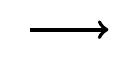
\begin{tikzpicture}
  \SetVertexNoLabel 
  \grCycle[RA=1.2]{8}
  \begin{scope}[rotate=45]
    \tikzset {
      VertexStyle/.append style = {
		    fill = white
      }
    }
    \grEmptyCycle[prefix=v,RA=1.2]{4}
  \end{scope}
\only<2-3>{
  \draw[->,ultra thick,line width=0.5mm] (2,0) -- (3,0);

  \grEmptyCycle[x=5,RA=1.2]{4}
}
\end{tikzpicture}%
\only<3-3>{
\caption {
  Vîrfurile albe (graful din stînga) formează o 4-mulțime de articulare.
  Suprimînd aceste vîrfuri obținem un graf (din dreapta) cu patru componenet conexe.
}
}
\end{figure}

\vspace{-2em}
}

\only<4->{
\begin{figure}
\centering%
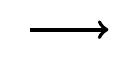
\begin{tikzpicture}
  \SetVertexNoLabel
  \grStar[RA=1.2]{8}

  \begin{scope}[rotate=45]
    \tikzset {
      VertexStyle/.append style = {
		    fill = white
      }
    }
    \grEmptyCycle[RA=0]{1}
  \end{scope}
\only<5->{
  \draw[->,ultra thick,line width=0.5mm] (2,0) -- (3,0);

  \grEmptyCycle[x=5,RA=1.2]{8}
}
\end{tikzpicture}%
\only<6->{
\caption {
  Suprimarea vîrfului alb (stînga) rezultă într-un graf (dreapta) cu opt componente conexe.
  Cu șapte componente mai mult decît cel din stînga. Vîrful alb este un vîrf de articulare.
}
}
\end{figure}
}

\end{frame}



\begin{frame}
  \frametitle{Mulțimi separatoare}

Așadar printre grafurile conexe sînt grafuri care pot fi ``rupte'' doar prin suprimarea unui vîrf sau a două vîrfuri, iar în altele pentru a le ``rupe'' este nevoie de a înlătura mai multe vîrfuri.\pause

Un fel de ``grad al conexității''.\pause

Noțiunea de $k$-conexitate

\end{frame}

\begin{frame}
  \frametitle{$k$-conexitate}

Un graf $G$ este \emph{$k$-conex}, $k\in\mathbb{N}$, dacă:
\begin{itemize}
  \item $|G|>k$;
  \item $G-U$ este conex pentru orice $U\subseteq V$ cu $|U|<k$.
\end{itemize}\pause

Cu alte cuvinte un graf este $k$-conex dacă are mai mult de $k$ vîrfuri și nu există mulțimi de articulare cu mai puțin de $k$ vîrfuri.

\end{frame}

\begin{frame}
  \frametitle{Exemplu: graful $W_9$}

\begin{minipage}{0.39\textwidth}
\begin{tikzpicture}
  \SetVertexNoLabel
  \grWheel[RA=1.5]{9}
  \SetVertexLabel
  \Vertices[unit=1.5]{circle}{s,t,u,v,w,x,y,z}
  \Vertex[Lpos=5,Ldist=.2cm]{p}
\end{tikzpicture}
\end{minipage}
%
\begin{minipage}{0.59\textwidth}
\begin{itemize}
  \item $W_9$ Conține vîrfuri de articulare?\pause
    \begin{itemize}
      \item Nu;\pause
      \item Deci este $2$-conex.\pause
    \end{itemize}
  \item $W_9$ Conține 2-mulțimi de articulare?\pause
    \begin{itemize}
      \item Nu;\pause
      \item Deci este $3$-conex.\pause
    \end{itemize}
  \item $W_9$ Conține 3-mulțimi de articulare?\pause
    \begin{itemize}
      \item Da, de exemplu, $\{p,v,t\}$;\pause
      \item Deci nu este $4$-conex.
    \end{itemize}
\end{itemize}

\end{minipage}

\end{frame}
  \frametitle{Mai multe exemple}

\begin{frame}
\begin{minipage}{0.49\textwidth}
\begin{figure}
\begin{tikzpicture}
  \SetVertexNoLabel
  \grWheel[RA=1.5]{13}%
\end{tikzpicture}
\caption{$W_{13}$ este 3-conex, dar nu și 4-conex}
\end{figure}
\end{minipage}\pause
%
\begin{minipage}{0.49\textwidth}
\begin{figure}
\begin{tikzpicture}[rotate=30]
  \SetVertexNoLabel
  \grCycle[prefix=a,RA=1.5]{7}
\end{tikzpicture}
\caption{$C_7$ este 2-conex, dar nu și 3-conex}
\end{figure}
\end{minipage}\pause

\begin{minipage}{0.49\textwidth}
\begin{figure}
\begin{tikzpicture}[rotate=30]
  \SetVertexNoLabel
  \grStar[RA=1.5]{8}%
\end{tikzpicture}
\caption{$S_9$ este ???-conex, dar nu și ???-conex} 
\end{figure}
\end{minipage}\pause
%
\begin{minipage}{0.49\textwidth}
\begin{figure}
\begin{tikzpicture}
  \SetVertexNoLabel
  \grComplete[RA=1.5]{8}
\end{tikzpicture}
\caption{$K_9$ este ???-conex, dar nu și ???-conex}
\end{figure}
\end{minipage}

\end{frame}

\begin{frame}
  \frametitle{Exemple extremale}

Ce putem spune despre $K_n$?\pause Dar despre $N_n$?\pause

Există grafuri 0-conexe?\pause Care grafuri sînt 1-conexe?\pause

Pentru a răspunde aceste întrebări vom considera negația condițiilor din definiția $k$-conexității și anume:\pause

Un graf $G$ nu este \emph{$k$-conex} dacă:
\begin{itemize}
  \item $|G|\leq k$ \alert{sau}
  \item există $U\subseteq V$ încît $|U|<k$ și $G-U$ nu este conex.
\end{itemize}

\end{frame}

\begin{frame}
  \frametitle{Exemple extremale}

\begin{itemize}
  \item $K_n$ este este 1-conex, 2-conex, ... și $(n-1)$-conex;\pause
    \begin{itemize}
      \item Însă $K_n$ nu este $n$-conex deoarce $|K_n|\not> n$.\pause
    \end{itemize}
  \item $S_n$, $n\geq 2$, este 1-conex;\pause
    \begin{itemize}
      \item $S_n$ nu este 2-conex întrucît are vîrfuri de articulare (de fapt doar unul).\pause
    \end{itemize}
  \item $N_1$ este $0$-conex (încercați să utilizați negația definiției pentru a arăta că nu este 0-conex);\pause
    \begin{itemize}
      \item $N_1$ nu este $1$-conex.\pause
    \end{itemize}
  \item $N_n$ este $0$-conex;\pause
  \item Graful $\emptyset$ nu este k-conex pentru niciun $k\in\mathbb{N}$.
\end{itemize}

\end{frame}


\begin{frame}
  \frametitle{Exemple extremale; Concluzii}

\begin{itemize}
  \item Orice graf conex netrivial este $1$-conex.\pause
    \begin{itemize}
      \item Un graf netrivial este 1-conex doar dacă este conex.\pause
    \end{itemize}
  \item Orice graf neconex și nevid este $0$-conex.\pause
  \item Orice graf nevid este $0$-conex.
\end{itemize}


\end{frame}

\begin{frame}
  \frametitle{Număr de conexiune}

Cel mai mare număr $k\in\mathbb{N}$ pentru care $G$ este $k$-conex se numește 
\emph{conexitatea} (sau \emph{număr de conexiune a}) grafului și se notează prin $k(G)$.\pause

Așadar: 
\begin{itemize}
  \item $k(K_n)=n-1$;\pause
  \item $k(G)=0$ dacă și numai dacă $G$ nu este conex sau $|G|\leq 1$;\pause
  \item $k(G)=1$ dacă $G$ are vîrfuri de articulare;\pause
  \item $k(G)\geq 2$ dacă $G$ nua re vîrfuri de articulare.
\end{itemize}

\end{frame}

\begin{frame}
  \frametitle{Mulțimi separatoare}

Fiind dat un graf $G$, o mulțime $F\subseteq E(G)$ se numește \emph{mulțime separatoare de muchii} dacă $G-F$ are mai multe componenete conexe decît $G$.\pause

Dacă se cunoaște că $|F|=k$ atunci $F$ se numește \emph{$k$-mulțime separatoare de muchii}.\pause

Dacă $k=1$, adică $F=\{e\}$, atunci $e$ se numește\pause{} \emph{punte}.

\end{frame}

\begin{frame}
  \frametitle{$\lambda$-muchie-conexitate}

Un graf $G$ se numește \emph{$\lambda$-muchie-conex}, $\lambda\in\mathbb{N}$, dacă:
\begin{itemize} 
 \item $|G|>1$;
 \item $G-F$ este conex pentru orice $F\subseteq E$ cu $|F|<\lambda$.
\end{itemize}\pause

Cu alte cuvinte $G$ este $\lambda$-muchie-conex dacă nu este trivial și nu conține mulțimi separatoare de muchii din mai puțin de $\lambda$ elemente.
 
\end{frame}

\begin{frame}
  \frametitle{Exemple}

\begin{figure}
\centering%
\begin{tikzpicture} 
  \SetVertexNoLabel 
  \grPath[Math,prefix=u,RA=1.2,RS=0]{4}  
  \grPath[Math,prefix=v,RA=1.2,RS=1]{4}
  \grPath[Math,prefix=x,RA=1.2,RS=2]{4}  
  \EdgeIdentity{u}{v}{4}
  \EdgeIdentity{v}{x}{4} 
  \SetVertexLabel
  \Edge[label=$f$](x3)(v3) 
  \Edge[label=$e$](x3)(x2)  
\only<2->{
  \draw[->,ultra thick,line width=0.5mm] (4.2,1) -- (5.3,1);

  \begin{scope}[xshift=6cm]
    \SetVertexNoLabel 
    \grPath[Math,prefix=u,RA=1.2,RS=0]{4}  
    \grPath[Math,prefix=v,RA=1.2,RS=1]{4}
    \grPath[Math,prefix=x,RA=1.2,RS=2]{3}  
    \EdgeIdentity{u}{v}{4}
    \EdgeIdentity{v}{x}{3} 
    %\SetVertexLabel
    \Vertex[x=3.6,y=2]{v}
  \end{scope}
}  
\end{tikzpicture}%
\only<3->{
\caption{Graf 2-muchie-conex (stînga), dar nu și 3-muchie-conex pentru că după suprimarea muchiilor $e$ și $f$ devine neconex}
}
\end{figure}
  
\end{frame}

\begin{frame}
  \frametitle{Număr de muchie-conexiune}

Cel mai mare număr $\lambda\in\mathbb{N}$ pentru care $G$ este $\lambda$-muchie-conex se numește \emph{număr de muchie-conexiune} a grafului $G$ și se notează prin $\lambda(G)$ (sau $k'(G)$).\pause

Din perspectiva ``conexității muchie'' conexitatea simplă se mai numește ``conexitatea vîrf''.

\end{frame}

\begin{frame}
  \frametitle{Exemple}

\begin{figure}
\centering%
\begin{tikzpicture} 
  \SetVertexNoLabel 
  \grPath[Math,prefix=u,RA=1.2,RS=0]{4}  
  \grPath[Math,prefix=v,RA=1.2,RS=1]{4}
  \grPath[Math,prefix=x,RA=1.2,RS=2]{4}  
  \EdgeIdentity{u}{v}{4}
  \EdgeIdentity{v}{x}{4} 
  
\end{tikzpicture}%
\pause
\caption{$\lambda(G)=2$, $k(G)=3$}
\end{figure}
  
\end{frame}

\begin{frame}
  \frametitle{$k(G)$ vs. $\lambda(G)$}

\begin{theorem} Pentru orice graf $G$ avem 
$k(G)\leq \lambda(G)\leq \delta(G)$
\end{theorem}\pause

Este evident că $\lambda(G)\leq \delta(G)$; dacă la un vîrf de gradul $\delta(G)$ înlăturăm toate muchiile incidente cu acesta numărul de componente conexe va crește cu 1.

\end{frame}

\begin{frame}
  \frametitle{Grafuri 2-conexe}

În cazul cînd un graf nu este conex acesta este format din mai multe componente conexe.\pause

Vrem să extindem noțiunea de componentă conexă pentru grafurile care nu-s 2-conexe.\pause

Adică, dacă un graf nu este 2-conex atunci el constă din mai multe ``componente 2-conexe''.\pause

Analogul este conceptul de bloc:\pause

Un \emph{bloc} al unui graf este un subgraf maximal conex și fără vîrfuri de articulare.\pause

Punctele de legătură între blocurile unui graf sînt vîrfurile de articulare.

\end{frame}

\begin{frame}
  \frametitle{Exemplu}
  
\begin{figure}
\centering%  
\begin{tikzpicture}
  \SetVertexNoLabel
  \grCycle[RA=1]{3}
  \grComplete[x=2,RA=1]{4}
  \grPath[x=3,RA=1,RS=0]{2}
  \grCycle[x=5,RA=1]{4}
\end{tikzpicture}  
\end{figure}\pause

Blocurile acestui graf sînt:\pause

\begin{figure}
\centering%  
\begin{tikzpicture}
  \SetVertexNoLabel
  \grCycle[RA=1]{3}
  \grComplete[x=3,RA=1]{4}
  \grPath[x=5,RA=1,RS=0]{2}
  \grCycle[x=8,RA=1]{4}
\end{tikzpicture}  
\end{figure}  

\end{frame}

\begin{frame}
  \frametitle{Blocuri}

\begin{theorem}
Pentru orice graf $G$ orice cilcu parține în întregime unui bloc. 
\end{theorem}\pause

\begin{proof}
Orice ciclu este un subgraf conex și fără vîrfuri de articulare.

Deci aparține unui subgraf maximal cu acestă proprietate.

Astfel de subgrafuri se numesc blocuri. 
\end{proof}


\end{frame}

\begin{frame}
  \frametitle{Blocuri}

\begin{theorem}
Fie $G$ un graf conex cu cel puțin 3 vîrfuri. Atunci următoarele sînt echivalente:
\begin{enumerate}
  \item $G$ este un bloc;
  \item Orice două vîrfuri din $G$ aparțin unui ciclu comun;
  \item Orice vîrf și muchie din $G$ aparțin unui ciclu comun;
  \item Orice două muchii din $G$ aparțin unui ciclu comun;
\end{enumerate}
 
\end{theorem}


\end{frame}


\begin{frame}
  \frametitle{Ilustrare}
\end{frame}


\begin{frame}
  \frametitle{Teoremele Menger}
 
Două sau mai multe lanțuri se numesc \emph{independente} dacă au cel mult două 
vîrfuri comune - capetele.\pause

\begin{theorem}[Menger 1927]\cite{diestel}
Fie $G=(V,E)$ un graf și $U,W\subseteq V$. Atunci numărul minim de vîrfuri care 
separă $U$ și $W$ în $G$ este egal cu numărul maxim de $(U,W)$-lanțuri 
independente.
\end{theorem}\pause


\begin{theorem}[Menger 1932]\cite{GTA}
Un graf $G$ cu $|G|=n\geq 3$ este 2-conex dacă și numai dacă între orice două 
vîrfuri există cel puțin două lanțuri independente.
\end{theorem}

\end{frame}

\begin{frame}
 \begin{proof}
{\em Suficiența.} Dacă între orice două vîrfuri ale lui $G$ există cel puțin 
două lanțuri independente atunci nici un vîrf al lui $G$ nu poate fi vîrf de 
articulare. Deci $G$ este $2$-conex.

{\em Necesitatea.} Fie $G$ un graf $2$-conex. Vom demonstra teorema prin 
inducție pe distanța $d(v,w)$ dintre două vîrfuri $v$ și $w$.

Fie $d(v,w)=1$, întrucît $G$ este $2$-conex reiese că $v$ și $w$ nu pot fi 
vîrfuri de articulare și evident muchia $\{v,w\}$ nu poate fi punte, ceea ce 
presupune că există un ciclu $C$ în $G$ care conține muchia $\{v,w\}$. Iată cele
două lanțuri independente căutate: $v,w$ și $vCw$.

Presupunem că teorema este adevărată pentru orice două vîrfuri cu distanța mai 
mică decît $k\in\mathbb{N}$. Fie $v$ și $w$ două vîrfuri cu $d(v,w)\geq 2$. Considerăm 
un $(v,w)$-lanț de lungimea $k$ și fie $x$ un vîrf care îl precede pe $w$ în 
acest lanț. Întrucît $d(v,x)<k$, din ipoteza inducției, pentru aceste două 
vîrfuri există două lanțuri independente $P$ și $Q$. Pe de altă parte, întrucît 
$G$ este $2$-conex, $G-x$ este conex și respectiv conține un $(v,w)$-lanț $P'$.
\end{proof}


\end{frame}


\begin{frame}
 \begin{corollary}
Dacă $G$ cu $|G|=n\geq 3$ este 2-conex atunci pentru orice două vîrfuri există 
un ciclu care le conține.
\end{corollary}\pause

\begin{corollary}
Dacă $G$ este un bloc cu $|G|=n\geq 3$ atunci pentru orice două muchii există 
un ciclu care le conține.
\end{corollary}\pause
\begin{proof}
Fie $e_1$ și $e_2$ două muchii. Subdividem aceste două muchii și notăm 
vîrfurile noi prin $v_1$ și $v_2$. Graful nou la fel este bloc și deci putem 
aplica corolarul de mai sus. Adică există un cilcu care conține aceste două 
vîrfuri. Dar aceste două vîrfuri nu alți vecini decît extremitățile mucgiilor 
$e_1$ și $e_2$. Deci și ele paarțin ciclului.
\end{proof}

\end{frame}

\begin{frame}
  \frametitle{Teorema Menger; Versiunea globală}

\begin{theorem}[Menger-Whitney]
Dacă $|G|\geq k+1$ este $k$-conex dacă și numai dacă orice două vîrfuri sînt 
unite prin cel puțin $k$ lanțuri indepenedente.
\end{theorem}

\end{frame}


\end{document}

